\documentclass[10pt]{book}

\usepackage{fourier}
\usepackage{fancyhdr}
\usepackage{color}
\usepackage{graphicx}
\usepackage{soul}

\pdfpageheight 8in
\pdfpagewidth 5in

\setlength\topmargin{-.344in}
\setlength\headheight{0in}
\setlength\headsep{0in}
\setlength\textheight{6in}
\setlength\textwidth{3.2472in}
\setlength\oddsidemargin{-.25in} % to make effective .5in b/c of .25 of binding
\setlength\evensidemargin{0in} % to make effective .5in b/c of .25in of binding
\setlength\parindent{0in}
\setlength\parskip{1em}

\newenvironment{fullpage}{%
  \begin{list}{}{%
    \setlength{\topmargin}{-1in}
    \setlength{\textheight}{8in}
    \setlength{\topsep}{0pt}%
    \setlength{\leftmargin}{-.6in}% take into account the .25" of binding
    \setlength{\listparindent}{\parindent}%
    \setlength{\itemindent}{\parindent}%
    \setlength{\parsep}{\parskip}%
  }%
  \item[]}{\end{list}}

\def\ck{\kern 1pt}
\def\phd{{\sc PhD}}

\sodef\chpso{\Large}{.1em}{.5em}{0em}
\sodef\secso{}{.05em}{.3em}{0em}

\makeatletter
\def\cleardoublepage{\clearpage\ifodd\c@page\else\thispagestyle{empty}\hbox{}\newpage\fi}

\def\@chapter[#1]#2{\cleardoublepage%
\refstepcounter{chapter}\addcontentsline{toc}{chapter}{#1}%
\chpso{\MakeUppercase{#1}}\\*
\rule[-2pt]{\linewidth}{.5pt}\vspace*{-9pt}}

\renewcommand{\section}{\@startsection{section}{1}{0mm}%
   {10pt}%
   {8pt}{\large\scshape\MakeLowercase}}

\renewcommand{\subsection}{\@startsection{subsection}{2}{0mm}%
   {6pt}%
   {6pt}{\normalfont\normalsize\itshape}}

\renewcommand{\subsubsection}{\@startsection{subsubsection}{3}{0mm}%
   {0pt}%
   {0pt}{\normalfont\normalsize\scshape\MakeLowercase}}

\renewcommand{\tableofcontents}{\cleardoublepage
\chpso{TABLE OF CONTENTS}
  \vskip0pt
  \rule[8pt]{\linewidth}{.5pt}
  \vspace{-3pt}
  \@starttoc{toc}}
\makeatother

\pagestyle{fancy}
\fancyhf{}
\fancyfoot[LE,RO]{\addvspace{10pt}\small\thepage}
\renewcommand{\headrulewidth}{0pt}
\fancypagestyle{plain}{%
\fancyhead{}
}

\begin{document}

\frontmatter

% 0th right page: blank
\thispagestyle{empty}
\mbox{}
\newpage

% 1st left page: blank
\thispagestyle{empty}
\mbox{}
\newpage

% 1st right page: promo
\thispagestyle{empty}
\mbox{}
\vfil\eject

% 2nd left page: blank
\thispagestyle{empty}
\mbox{}
\newpage

% 2nd right page: half-title
\thispagestyle{empty}
\begin{fullpage}

\includegraphics{2017-redbook-halftitlepage.pdf}
\end{fullpage}
\vfil\eject

% 3rd left page: blank
\thispagestyle{empty}
\mbox{}
\newpage

% 3rd right page: full-title
\thispagestyle{empty}
\begin{fullpage}
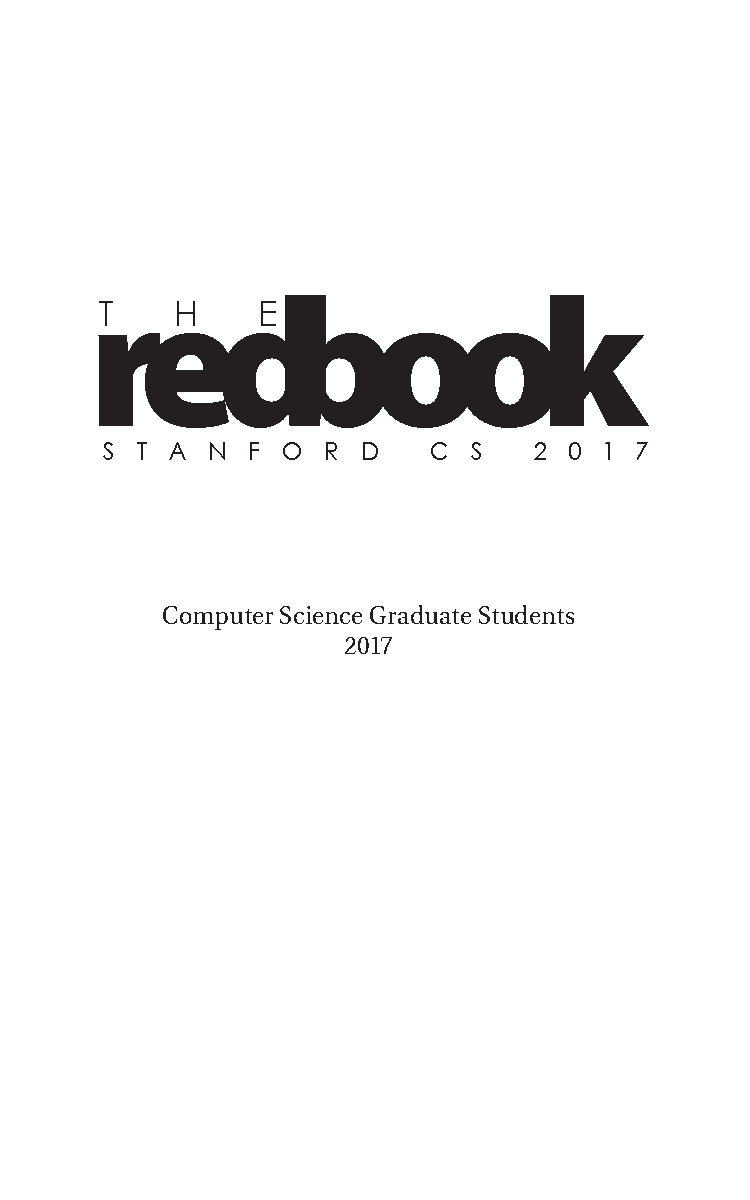
\includegraphics{2017-redbook-titlepage.pdf}
\end{fullpage}
\vfil\eject

% 4th left page: copyright, publication information
\vspace*{5in}
{\small
\noindent Published 2007, 2008, 2009, 2010, 2011, 2012, 2013, 2014, 2015, 2016, 2017\\*
Printed in the United States of America

\noindent Typeset with \LaTeX\ in Utopia, originally by Austen McDonald\\*
http://austenmcdonald.com
}
\thispagestyle{empty}
\vfil\eject

% 4th right page: dedication
\thispagestyle{empty}
{\Large\it Dedicated to$\ldots$}
\vskip 0pt
{\it\hspace{.5in} $\ldots$the incoming class of 2017. Best of luck!}
\newpage

% 5th left page: blank
\mbox{}
\thispagestyle{empty}
\newpage

% 5th right page: acknolwedgements: put all authors and contributors here, in
% alphabetical order, grouped by year
\chpso{ACKNOWLEDGMENTS}
\vskip0pt
\rule[8pt]{\linewidth}{.5pt}
%\vspace{-3pt}
{\bf 2007}\\*
Ioannis Antonellis\\*
Billy Chen\\*
Mike Houston\\*
Jeff Klingner\\*
Austen McDonald\\*
Adam Oliner\\*
Doantam Phan\\*
Ron Yeh\\*
\vspace{0.2in}\\*
{\bf 2008}\\*
Chand John\\*
Austen McDonald\\*
Adam Oliner\\*
Rachel Weinstein\\*
Leslie Wu\\*
\vspace{0.2in}\\*
{\bf 2009}\\*
Kathi DiTommaso\\*
Chand John\\*
Austen McDonald\\*
Adam Oliner\\*
Verna Wong\\*
Leslie Wu\\*
\vspace{0.2in}\\*
{\bf 2010}\\*
Kathi DiTommaso\\*
Chand John\\*
Austen McDonald\\*
Adam Oliner\\*
Verna Wong\\*
Leslie Wu\\*
\vspace{0.2in}\\*
{\bf 2011}\\*
Kristen Babineau\\*
Helen Buendicho\\*
Steven Whang\\*
Verna Wong\\*
\vspace{0.2in}\\*
{\bf 2012}\\*
Kristen Babineau\\*
Helen Buendicho\\*
Ankita Kejriwal\\*
Manolis Savva\\*
Verna Wong\\*
\vspace{0.2in}\\*
{\bf 2013}\\*
Helen Buendicho\\*
Ankita Kejriwal\\*
Manolis Savva\\*
Jayanthi Subramanian\\*
Verna Wong\\*
\vspace{0.2in}\\*
{\bf 2015}\\*
Tudor Achim\\*
Henry Qin\\*
Verna Wong\\*
\vspace{0.2in}\\*
{\bf 2017}\\*
Collin Lee\\*
{
\setlength\parskip{0em}
\tableofcontents
}

\mainmatter

\section{\secso{What is This?}}
The Redbook is the attempt of a few \phd\ students to pass on bits of wisdom
and frank advice to newer students in the hope that the next generation avoids
their missteps. It lives online at http://github.com/austenmc/theredbook.

\textbf{tl;dr}

Meet as many of your peers as possible. Within them lies all the knowledge in
this book, insights to unblock you when you are stuck, empathy to support you
when you despair, and energy to bolster you when you fatigue.

\chapter{The Basics}

\section{\secso{Three Things to Know}}
\begin{enumerate}
\item Academia is a business, and graduate student is a job title. From Azuma:
``Academia is not the Real World and does not work in the same way that the
ordinary corporate world does. However, it is a business nonetheless and as a
graduate student, you must treat it that way. Graduate school made a lot more
sense and became much easier for me after I realized this. If you think of
graduate school as an `Ivory Tower' free of politics, money problems, and
real-world concerns, you will be severely disappointed.''
\item Remember you're here to get a \phd. Especially if you come straight from
college, the apparent lack of requirements may cause you to not take school
seriously. Have fun, just don't have {\it too much fun}. Have
a plan for completing your degree in a timely fashion.

\item Acquire good advice by chatting with senior graduate students behind
closed doors; they will be more open and honest.

\end{enumerate}

\section{\secso{PhD Requirements}}
In your first quarter, {\it don't drift}. Make yourself aware of the \phd\ requirements:

http://cs.stanford.edu/academics/phd/phd-requirements

These include enrolling in CS300 and CS499 during your first year, completing your Breadth Requirements and applying for candidacy by the end of your second year, passing your quals by the end of your third year, and submitting the Reading Committee Form and Thesis Proposal Form by the end of your fourth year. Many students get credit for classes they have already taken as undergrads. On the other hand, taking classes in the Breadth Requirements can be a good opportunity for learning new topics.  You can find more details about the PhD program at this address:

http://cs.stanford.edu/academics/phd

If you have any questions don't hesitate to visit Jayanthi or Helen at the student services office (Gates 196).

\section{\secso{The Rotation System}}
The CS department has a rotation system, which is a great opportunity to experience multiple advising styles and research group dynamics. The goal of the rotation system is to find a permanent advisor by the end of spring quarter of your first year. Set up your winter (and spring) rotations as soon as you can in the fall quarter. Attend the CS300 seminars to hear about current research projects. Here is some useful information and advice coming from a survey of students who went through rotations in the last two years.

\begin{itemize}

\item Many students felt that going through rotations gives them more confidence when choosing an advisor, even if they ended up choosing the advisor they would have chosen without rotating. In many cases, students changed their mind and were happier for having done so.

% \item Through rotations you get to know more faculty and students. These are valuable relationships that are helpful even if you don't end up in the same group, so try to keep in touch after you are done with your rotations. You will benefit from getting different perspectives on ways of doing research.

\item Try to reach out to the students of your potential rotation advisor before you decide to rotate, and ask very specific questions such as the number of hours the advisor meets with them each week and how responsive they are to office visits and emails.  You may also want to reach out to previous rotation students as well.  You can find who rotated with whom in this address:

https://cs.stanford.edu/internal/student-info/phd-rotation-statistics

\item Try to meet with your rotation advisor in advance of the rotation to work out the details of
    your project. In the same meeting, you should try to agree on the expectations for the project, as well as inquire about whether the advisor is still taking students. Some advisors will take students for rotations but not necessarily have a spot in the lab for you.

\item One quarter is not much time. It is important to have this time frame in mind and decide on a well-defined project. Establishing realistic goals with your advisor is also important, particularly in minimizing the amount of ``bleed over'' of rotation projects into subsequent quarters.

\item The student survey revealed that student happiness with the rotation experience was highly correlated to the frequency of meetings with the rotation advisor. Meet with your rotation advisor as frequently as possible to keep them involved in your project and ask for feedback. Other highly correlated student responses are in Table~\ref{tab:surveyTable}.

%In some cases (i.e. conference/journal deadlines) this may be unavoidable, but both parties should work to minimize it as much as possible.

%\item Try to work with a more senior student during the rotation. You will get more direction, mentorship, and an additional conduit for learning about what it is really like to work for a particular faculty member. Having two or more rotation students work together on a project can also be effective.

\item It can be valuable to do one rotation with a faculty member in an area that is a little out of your comfort zone, but still relevant to your interests. Working with someone outside of CS is also possible, but meet with someone in the CS student services office to figure out how you will get funded.

\item If you are thinking about aligning early, chat with Prof. Ousterhout, the Ph.D program director, or a staff member in the CS student services office first about the decision.

\end{itemize}

\begin{table}[ht]
\footnotesize
\begin{center}
\tabcolsep=0.05cm
\begin{tabular}{r|c}
   & \parbox[c]{1.5cm}{\centering Student happiness}\\
  \hline
  Meeting frequency with advisor & 0.49 \\
  Meeting frequency with other students & 0.29 \\
  Student believes sufficient feedback received & 0.57 \\
\end{tabular}
\caption{Correlation table for rotation experience survey. Responses were from 31 PhD students who rotated in 2010-2012. The values are Spearman's coefficients and are all statistically significant with $p<0.05$.}
\label{tab:surveyTable}
\end{center}
\end{table}

%\begin{figure}[h!]
%  \centering
%    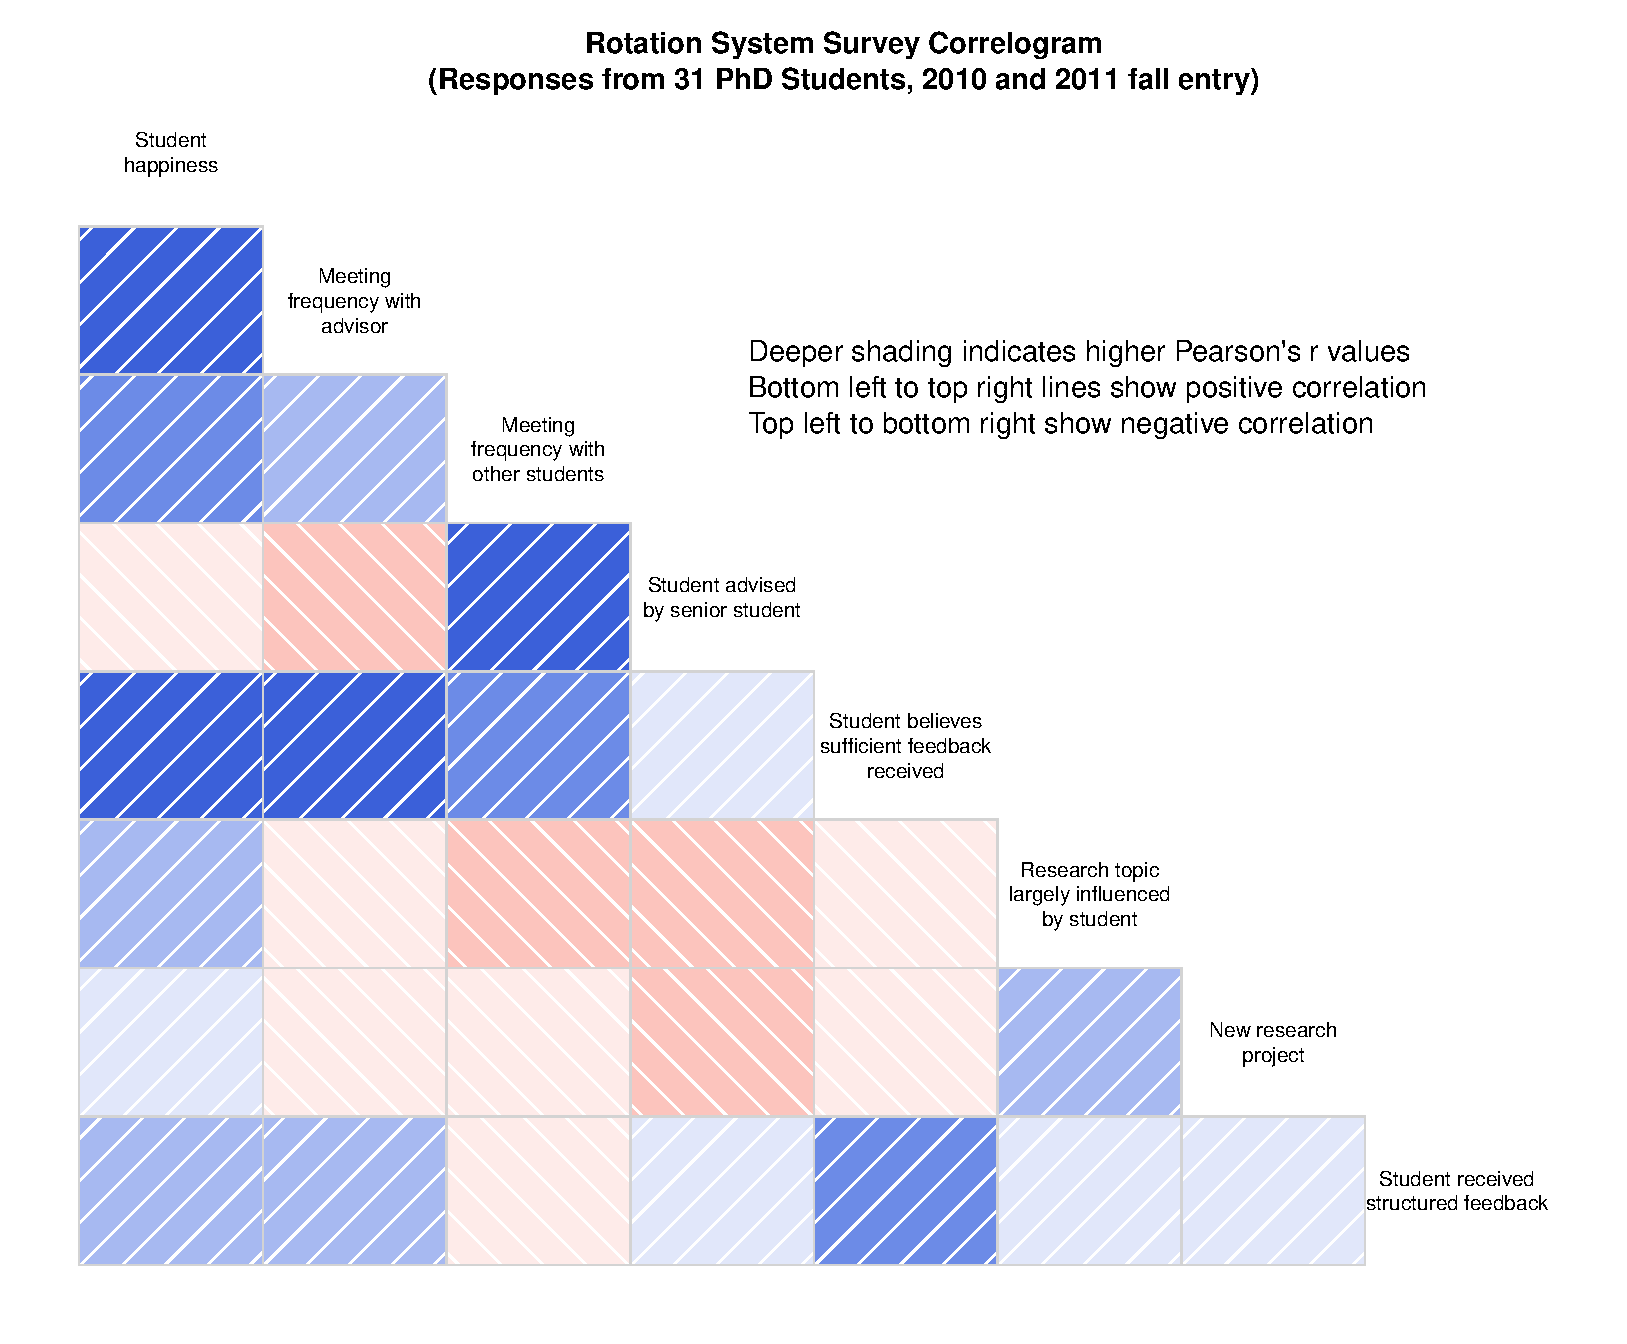
\includegraphics[width=1.0\textwidth]{surveyCorrelogram.pdf}
%\end{figure}

%When working with a professor, don't just attend meetings: work on an existing project with
%more senior grad students for a chance to be mentored and learn by
%their example. (Try to pick a good project!) Take a lesson from other fields,
%which have students rotate through different labs in their first year. Even if
%you don't end up with that advisor, you've gotten research experience,
%perhaps credit on a paper, and a professor in the department who knows you. If you have
%difficulties later in the program, for whatever reason, it is crucial to have a
%professor who knows you and who will go to bat for you.

\section{\secso{Advisors}}
\subsection{Choosing an Advisor}
{\it The choice of advisor is by far the most important decision you'll make}, by any
order of magnitude.

It will completely control your grad school experience and
will affect your post-grad-school career, especially if you want to
continue in academia.

\subsubsection{Other Students' Experiences. }
The best way to learn about an advisor is to chat with current
members of that professor's group behind closed doors. They'll give you the
real information about a professor, from inspiring tales to horror stories.
Both exist. Ask them about the topics below.

\subsubsection{Funding. }
When choosing an advisor, you need to understand their funding situation. Don't
be afraid to discuss this candidly---it's the only way to avoid
misunderstandings. Without funding, you will be supported by the department,
which means you have to be a course assistant ({\sc ca}). You don't want this
to happen because {\sc ca}ships take a considerable amount of time away from
research. A 50\% {\sc ca}ship covers your tuition and stipend, but generally
requires $\approx 20$ hours per week of work from you. Although 25\% {\sc ca}ships
exist, the common wisdom is that you will be working almost as much as the 50\%
{\sc ca} for less money. Another source of funding is industrial fellowships
(Microsoft, {\sc ibm}, {\sc nvidia}, {\sc ati}). The department usually controls
who gets to apply for these fellowships or it is limited to one applicant per
professor.

Keep in mind the following questions: Are there active grants that can
support your specific research project as a 50\% {\sc ra}? How many quarters of
support are these grants? Are they renewable? What is the criteria under which
they can be renewed? Are your professors actively writing more grants for the
future? If not, will they help you write a grant (it's good practice, in any
case)?

Have a candid talk with your advisor to avoid being forced to {\sc ca} quarter after quarter
while struggling to produce research. If this
does happen to you and you still graduate, however, turn those
lemons into lemonade by earning a Distinction in Teaching. A Distinction in Teaching is earned by completing the equivalent of 10 units in TA/TF (teaching assistant / teaching fellow), including at least one quarter as a TF with primary responsibility for organizing and teaching a course. The units must include at least one course at each of the 100, 200 and 300-plus levels.

\subsubsection{Advisor Age. }
A young (pre-tenure) advisor will be hungry for results and will be
closely involved with your work. They are likely to
closely monitor the relevant conferences and will be
well aware of related work. This may appeal to you.
The downside is that they may fail to make tenure,
which could screw up your grad school career.

An old advisor will have fame, experience, and contacts.  They are a safer bet
than a pre-tenure professor since they aren't going anywhere, and many have
reliable funding. On the other hand, older, successful professors {\it
sometimes} aren't hungry for success anymore, and may be only superficially
engaged in the research of their students, leaving them feeling adrift.

\subsubsection{Recent Publishing Record. }
If you want to pursue an academic career at a top-tier school, you'll need
several high-quality first-author papers. Look at how many papers the
professor's current students have published in the past few years, and at what
conferences. This is an indicator of where the professor
stands with respect to the earlier point: are they still hungry to achieve
success, or are they resting on their laurels?

Aside from this question of hunger, professors also differ from
each other with respect to how they approach conferences; some publish
papers three times more often than others. Of course, paper quality matters
more than quantity, so use Citeseer, ACM Digital Library, or Google Scholar to see how often the
professor's recent papers are cited, as an indicator of how well their work is
received by their research community.

\subsubsection{Advising Style. }
Many will suggest you ask if a professor is ``hands-on'' or ``hands-off.''
These terms are not very meaningful because advisors often vary their time
investment from quarter to quarter depending on the timing of research
deadlines, whether they are teaching or not and the number of external
collaborations they are maintaining at any given time. More useful metrics are
the frequency with which they meet you (which can sometimes be lower than
scheduled), whether they are available to unblock you outside of official
meetings, and how their students describe them.

On the last point, most students will not say anything explicitly negative
about their advisor, but a lack of strong enthusiasm in recommending their
advisor can sometimes be a red flag.


%Unless you lean strongly toward one or the other, stick to other metrics when picking
% an advisor. % Be wary of professors at either extreme (talk to senior grad students).



\subsubsection{Group Composition. }
Find an advisor with several current students, since their body of
knowledge and experience will be of great benefit. Many groups work
like an apprenticeship: young students join existing projects to learn from the
older students, and, as they get more experience, they will strike out in their
own directions.

If all the current students are near graduation and there are no younger
current students in the pipeline, this could be a problem.

% Be wary of advisors with large groups (15+ students), because you'll
% get much less face-time than with only 5--10 students.

\subsubsection{Industry Contacts. }

Industry contacts are key in systems-related fields.  It is often hard to do
compelling research in a systems area without collaboration with industry
partners.  Do the professor's students work
for companies that excite you? Do the advisor's current students often do
consulting or summer internships in industry?

\subsection{Switching Advisors}

We do not recommend switching advisors after your second year, but it has
been done. If you want to switch, simply have a candid conversation with your
advisor; be honest and try to leave on peaceful terms.  Notify the \phd\ Program
Office if you switch advisors.

\subsection{Talking with your Advisor}

The role of your advisor is to provide `advice'. If you disagree, talk about it. Disagreements
may arise regarding research direction, summer plans, or even funding.

Talk to your advisor often, at least once a week. There are several
topics you may need to discuss during your \phd:

\begin{itemize}
\item {\it Be explicit about expectations.} How often does your advisor
expect you to publish? Specifically, what about the upcoming {\sc foo-bar}
conference? If you know your advisor's expectations, you are less likely to disappoint.

\item {\it Make meetings count.} Come to meetings
prepared with a plan of what to talk about, questions, etc., and leave with a
clear idea of what you'll do before the next meeting.

\item {\it Paper author order.} Credit for a research paper is determined by author order;
some groups encounter strife because there is no clear ordering policy.
Discuss it with your advisor ahead of time, rather than waiting until the paper is complete.
Likewise, beware of working on projects
with students on the same graduation schedule as you, as you
may both want first authorship on the same paper. When you are a senior student,
work with junior students to avoid these problems.

\item {\it Theses from large projects.} Large, multi-year projects can
involve an unknown number of graduate students, but usually produce a finite
number of theses. If you get involved in one of these projects,
discuss what part of the project can be used for your thesis. If that can't be
determined within the first few quarters, you may want to find a new project.
\end{itemize}

\section{\secso{Teaching}}

One requirement of the \phd\ program at Stanford is to complete at least 4
units as a course assistant (CA) or teaching fellow (TF) for courses in
Computer Science that are numbered 100 or above. For more information, see the
\phd\ requirements.

Be very cautious about signing up to TA for large classes taught by hands-off
professors. Always consult former TAs to get a good idea of the
professor's teaching style and his or her expectations (or lack thereof) of
TAs.

% Try to satisfy half of this requirement early on by being a CA for a class by your second year. A typical default is to teach one of your advisor's classes. It can also be good to diversify by teaching a class outside your research area and with professors other than your advisor.

\section{\secso{Funding}}

Funding is vital. Have candid talks with your advisor about it
so you can ensure support through your entire graduate career with minimal
distraction from your research. Your happiness and progress are correlated with
funding. Grad students with funding tend to be pretty
happy, but, without funding, grad life can be pretty miserable. Most students
find their thesis topic by working in an area or project that provides
them funding.

Every quarter you need 50\% of support. Funding comes in percent units,
usually 50\% or 25\%. Ideally, you are a 50\% Research Assistant ({\sc ra}),
funded under a grant from a government agency ({\sc doe}, {\sc dod}, {\sc nsf})
or a private organization, and working on an interesting topic.

You may be lucky and have a fellowship from Stanford, {\sc nsf}, {\sc ndseg},
Hertz, or some other group that covers you for three to five years. If you're
really lucky, you have two fellowships, one of which may be deferrable. If it's your
first year and you don't have a fellowship, you should apply for {\sc nsf},
which is still open to graduate students in their first and second year. There are
also one-year fellowships from companies like Microsoft, Intel, {\sc ati},
{\sc nvidia}, and Yahoo.  Other fellowships are offered by {\sc ibm}, the Ford
Foundation, {\sc npsc}, {\sc nasa}, {\sc llnl}, and {\sc aauw}.

If you're not on a grant or fellowship, then you're a Course Assistant ({\sc
ca}). Being a {\sc ca} requires $\approx 20$
hours a week of work. Do not be a long-term {\sc ca}. You will be unable to do enough research
to keep your advisor happy, and so you continue on as a {\sc ca}
in a vicious cycle.  If you have to {\sc ca}, ask the senior
grad students which courses require less than 20 hours
of work. A rule of thumb might be to avoid intensive programming project
courses like Operating Systems.

\subsection{Grants}

Grants are given to your advisor and your advisor employs you as an {\sc ra}. It is
rare, but not unheard of, for a professor to cut a student's funding.
They are required to give a one quarter notice so that you
have time to scramble to find other funding. This is something that should not
happen if you are having candid talks with your advisor about your
progress.

You should know what grant you are on, if it is renewable, and what the
criteria are for renewal. You should also know if your advisor is applying for
other grants from the {\sc nsf}, {\sc dod}, {\sc doe}, or whomever. Try to
help write the grant. If you want to be faculty in the future you
should know how to write a grant. If your advisor is not writing a
grant, you should be concerned. In this case, ask your advisor if they will
help you write a grant.  You can go to the {\sc nsf} website and look at the calls.

\subsection{50\% vs. 25\% CA}

Avoid a 25\% {\sc ca} (Course Assistantship). You usually do
nearly the same amount of work as a 50\% {\sc ca}, which fully funds you for
the quarter. As a 25\% {\sc ca}, you'll need to find another source of 25\%
funding (possibly a 25\% {\sc ra} with a professor who is not your advisor).

\subsection{50\% vs. 25\% RA}

Most {\sc ra}ships are 50\%. You are usually an {\sc ra} under your
advisor. Sometimes, people take an {\sc ra} position with someone else
to have support.  If this happens to you, minimize the impact
on your research by finding an {\sc ra} position that is somewhat related to
your research (e.g., kickstart a collaboration between your advisor and another professor).
Sometimes, an {\sc ra} under another professor may have you writing code for some group
in the university that needs it.
Students in the {\sc ee} department tend to know a little more about doing
{\sc ra}ships for PIs other than one's primary advisor, so try asking one of them.

\subsection{Fellowships}

A fellowship can be a double-edged sword. It's great to have long-term funding
with few or no strings attached, but the lack of quarter-to-quarter
accountability for funding can often lead to drift, especially in the case of a
hands-off advisor. Celebrate, but beware!

A fellowship can enable you to work
with the advisor you want to work with, because advisors tend to welcome
a student who comes with funding.

\subsection{Consulting}

Officially, students may consult for other companies for one day a week. It's a nice
way to make money and may not require too much time. However, international students
on full assistantships (50\% research or teaching appointments, for 20 hours of work
per week) may not be employed for any additional hours of work during the academic year
(more information available from the Bechtel international center).

\subsection{Summer Internships}

Internships are a great source of extra spending money, a valuable way to
hook into industry research, and a way to get ideas for a thesis. Spend at least
one summer at an industry research lab early in your graduate career.
Students have taken their summer
internship at an industry research lab (e.g., Microsoft Research) and
turned it into a thesis. Your advisor may have contacts and be able to recommend
internships. Some good places are Microsoft Research, Microsoft
Research Asia, Yahoo Research, {\sc hp} Labs, {\sc parc}, or
your advisor's company.

Faculty vary widely in their sentiment towards summer internships, so
if you are interested in doing multiple internships, you should have that
discussion up front with your advisor to ensure that you know how they feel
about it.

\subsection{Unrestricted Funds}

Grants are reserved for particular purposes and projects. So, you (usually)
can't get money from the {\sc foo} pot unless you work on the {\sc foo}
project. If you are lucky, however, your advisor may have some unrestricted funds to cover you. Unrestricted funds are often coveted, so don't rely on this.

\subsection{TGR}

If you're in your last year, have completed 135 units of coursework and all your milestones except for your orals and dissertation, you can make your fellowship money stretch further
by going {\sc tgr}, which reduces the amount of tuition.
You can technically only stay on {\sc tgr} for a year, but this rule has not yet been enforced by the university.

\subsection{Graduation Quarter}

If you need just one more quarter, the University Registrar's Office allows
you to register for a
graduation quarter which costs very little (\$100 plus fees). If you've saved up some
money and really are on your last quarter, you can take this option. If it proves not to be your last quarter, you can apply (or reapply) for TGR status.

%\section{\secso{Breadth Requirement}}
%
%Starting from 2010, students are required to pass the Breadth Requirements. Most of the students like it better than the previous Comps Requirements, and many get credit for classes they have already taken as undergrads. Details on passing the Breadth Requirements can be found at
%
%https://cs.stanford.edu/degrees/phd/Main/AcademicRequirements
%
%Focus on completing the Breadth Requirements, along with finding an advisor, in your first year. You must complete your Breadth Requirements by the end of your second year in order to file for candidacy.


\section{\secso{How to do Research}}

An undergraduate degree is about doing well in classes: someone tells you
what to do and how to do it. In graduate school, you are solely
responsible for setting your daily schedule, finding the right project to work
on, and figuring out how to accomplish it. This uncertainty may contribute to
a stressful existence while you adjust. There may be long stretches of
time when you doubt whether your work will be fruitful.

What follows are tips on how to avoid this uncertainty. Note that these tips
are rules of thumb and it is really up to you and your advisor to decide what
research looks like for you.

\subsection{Read Papers}

It is critical to read {\it lots} of papers in your area, and specifically on
your research topic. What if you don't like to read papers? Then, at
the very least, {\it skim} lots of papers.

\subsection{Talk With People}

Conversations make you smarter. They help you look at problems from different
perspectives, hone your arguments, refine your terminology, explore alternative
solutions, and uncover existing approaches. Chat with professors, other
graduate students (even outside your area), and anyone else who will give you
the time of day. Not only will this improve your research, but more people will
know you and what you are doing. Make sure you are listening at least as much
as you are talking.

Bounce your ideas off other colleagues. If they like your work, great. If not,
ask them why and improve your work based on their feedback.

\subsection{Be Goal-Oriented}

When deciding on research projects, be goal-oriented. Do not waste your time
working on projects that lead nowhere. Ask yourself, ``Will this project lead to
a paper? Which conference will I submit it to? Is it a chapter in my
thesis?'' Do not work on a project simply because it's cool.

\subsection{Set Deliverables and Discuss with your Advisor}

A project will span weeks, if not months or years. It is easy to become
distracted or discouraged. Set weekly goals. Turn these goals into
deliverables that you can share with your advisor and colleagues. If
you're going the wrong direction, the early feedback will help you get back on
track.

\subsection{Time Management and Procrastination}
Some (read:\ many) of us find it challenging to manage our schedules. If you really
need to get work done, consider techniques to avoid wasting time. If you close
your office door or wear headphones, fewer folks will bother you. If your office
is too loud, consider switching offices or working in the campus libraries.


\section{\secso{Quals}}

Quals is the milestone exam that tests the ``depth'' of your knowledge in your area. Some
folks take it their second year, some take it their third. Ideally, you should
pass quals on your first attempt. Officially, it's 100\% {\sc ok} to fail
your first time and then pass your second. It's possible but rare to take quals three
times, but your advisor better be loving your research, and you will go through
a petition process.  In the past ten years, no one has taken quals more than
three times, and roughly two students have taken quals exactly three times.
Students have left with a Masters after failing twice; other students have
passed on the third try, generally based on whether their advisor likes what they
are doing.

%In general, orals are ``better'' than written exams; the questioner can tease
%out the answers, whereas on a written exam there is no back-and-forth. Form
%study groups and try your best to pass on the first try.


\section{\secso{The Thesis}}

Theses vary between disciplines and even advisors. Your thesis should be
modeled after others in your area; grab some examples and discuss the structure
with your advisor. One rule of thumb is to have a few papers on a single topic
(approximately 3 in Graphics or {\sc hci}, for example), which then become the
main chapters of your thesis. One strategy for pushing ahead on your thesis is
to present your advisor with a proposed outline. This allows the both of you to
discuss what, if anything, may be missing from your research and can allow you
to target your work so that you can graduate in a timely manner.

\subsection{Committee}

You will need a thesis committee for your Thesis Proposal, your Oral Defense, and to read and sign your thesis. Pick committee members who will provide timely feedback.  If possible, meet with them somewhat regularly to update them on your progress to ensure everyone is on the same page. Also, make sure your reading committee will have time to read and sign your thesis.

\subsection{Proposal}

Your Thesis Proposal is a great time to formally solicite feedback from your committee. Proposing earlier rather than later can be extremely helpful.  You don't want your committee to be surprised at your defense about the direction you are taking for your thesis!  It is better to hear objections 12 months before your defense than the day of.

\subsection{Defense}

Your advisor shouldn't let you schedule a defense until you are ready. Most
people defend after having written some (but not all) of their thesis. Schedule
your orals two to three months in advance. Don't forget to bring food. Catering
means one less thing to worry about.


\subsection{Writing}

Thesis lengths vary from under a hundred pages to as long as several hundred pages. Some
advisors are comfortable with a ``stapled thesis,'' which is merely the papers
you've written with transition paragraphs between them. Other advisors
want the thesis to stand on its own as a treatise on a subject; this
requires rewriting.

This may also be a good thing to find out about when choosing an advisor.


\chapter{Health and Happiness}

\section{\secso{You Are An Asset}}

A graduate student costs more than \$100{\sc k/yr} to fund, including tuition,
stipend, office space, computing equipment, and travel expenses. You are an
enormous investment. A graduate student who is unable to do research (due to
{\sc rsi}, depression, or other physical or mental health issues) is a waste of that
money. Your advisor is likely to accommodate your needs where your well-being is
at stake. Recognize your value, and put your health above all else.

\section{\secso{Mental Health}}

A \phd\ can be a high-stress, low-social-interaction environment that can lead
to a variety of mental issues, including anxiety and depression.

Keep in mind that if you're stressed or feeling worried about the uncertainty
of grad school, other students are as well. You're not alone. Talk to
other students about it, it will make you feel better.
Counseling and Psychological Services ({\sc caps}), an arm of Vaden
Health Center, can provide additional help with mental health.

%The \phd\ Comic Strip has a forum populated with graduate students
%from around the world, which can be a great source of support:
%
%http://www.phdcomics.com/proceedings/

\section{\secso{Physical Health}}

Although we aren't medical doctors, we think that regular exercise is great for
reducing stress (and much more!). Take advantage of the Stanford athletic
facilities; apart from the gym, there are classes in tennis, swimming,
climbing, yoga, golf, volleyball. You also happen to be in the Bay Area:
there is skiing a few hours away, surfing in Santa Cruz, hiking and
climbing in Yosemite, and good weather year round.

Eat well. The free food around Gates is not
the healthiest.

Speaking of free food, you should certainly subscribe to the
\verb+gates-food@lists+ email list. Whenever free food is lying around Gates,
someone emails this list with a description. Remember to bring your own plate.

\subsection{RSI}

You probably do a lot of typing, and you may develop {\sc rsi}.
Educate yourself about ergonomics. Consider getting an ergonomic keyboard
(Kinesis Advantage or Kinesis Maxim or Goldtouch). Some students use Workrave which monitors typing
and mousing behavior and reminds you to take breaks every once in a while.
Students report that this has significantly improved their {\sc rsi}. The
default settings are appropriate if you're already experiencing pain (obey the
limits set by the program). If you just want to be preventative, set it to be less strict.

\section{\secso{Activities and Social Life}}

Join activities to meet people, gain life experiences, add
structure to your life, and maintain good physical and mental health.
At Stanford, there are student-run organizations
for just about every interest (e.g., swing dancing, juggling, hiking).
Top-notch instructors teach classes like golf, languages, social
dance, music, photography, and art.  Some students play intramural
sports, join larger clubs like Taekwondo or Wushu, join Stanford Outdoors
clubs, or do various kinds of dance, including Viennese Ball or the
Stanford Ballroom Dance Team.

If you live on campus, your residence has Community Associates (CAs) whose
main job is to provide social activities for you.
Rains has the most events, Lyman has many, and Escondido Village has some.

Stanford is located near a huge variety of off-campus destinations including
San Francisco, Yosemite, and Napa Valley.  The Graduate Life Office
(http://glo.stanford.edu) can help you find information on specific activities.

Get to know people in your research lab and department.  You will spend a lot
of time with them. When your code is broken right before
your thesis is due, these people will both want to help you and
know how to help you.

Start meeting people early: you will only grow busier.

\chapter{Department}
\section{\secso{Paperwork and Pitfalls}}
There are several types of paperwork that matter. They generally deal with
getting paid and completing your \phd\ milestones.

When you pass your Breadth Requirements, file your candidacy form so you get a
pay increase. If you have some strange advising situation (e.g., your advisor is
not natively {\sc cs} or has a joint appointment with another department),
make sure it goes through.

Before each quarter, secure funding. If you are {\sc ra}ing,
sign a form with your advisor's admin.

After you do your Thesis Proposal, there is a Thesis Proposal form.

When you near the end of your \phd, fill out a form for
your Reading Committee, and one to schedule your Oral Examination.

During the last year, you can go {\sc tgr} to save your lab money.

Many of the forms are at the addresses below:

http://cs.stanford.edu/academics/phd/graduate-student-forms

http://studentaffairs.stanford.edu/registrar/forms/grad

\chapter{Life After Grad School}

\section{\secso{Doing Something Else}}

About 7.5\% of \phd\ students drop out to pursue other interests. Some leave
with a Master's degree, others without. There are legitimate reasons for each
decision.  If you want to be faculty, or if you want to do research in the
future, you need a \phd. However, you may be unable to work with your advisor,
unable to find an advisor to work with, or disillusioned with the research
process.  There is an opportunity cost to staying in graduate school: we can
make very good salaries working in industry. (If you estimate a salary as
\$100{\sc k} and a graduate student stipend as \$30{\sc k}, \$70{\sc k} is what
you're ``giving up'' annually to be here.) There is also a cost to leaving
graduate school. Be clear with yourself about why you are still in the program
or why you want to leave. Before you make a final decision about leaving the
program, have a conversation about your decision with someone in the Student
Services office (Gates 196). There might be other options for you to consider.
If you do leave, try not to burn any bridges.

\section{\secso{Working in Industry}}

The Computer Forum (forum.stanford.edu) is a great in-house resource for
finding a job in industry. The Forum is a group of businesses interested in
supporting the CS department, probably because they get primo access to hires
from Stanford. Every year, they host career fairs, hold informative lunches with
local and global companies, and sponsor career-building events.

\section{\secso{Becoming Faculty}}

At most 15-20\% Stanford \phd\ graduates go on to faculty careers.  This is a
lower percentage than at other schools because of Stanford's strong industry
ties. As with much of grad school, successfully preparing for and landing a
faculty position won't just happen: you must take the initiative.

\subsection{Kinds of Faculty Positions}
Only about 5\% of Stanford \phd s (one or two students in your entering class) will end up
in a job that resembles their
advisor's tenure track position at a top-5 {\sc cs} department. Others will end
up lower on the ranking totem-pole or in other kinds of academic jobs. If you
are interested in academia, you should think about the basis for your interest.
Is it doing research?  Freedom to follow your interests?  Advising students?
Teaching?  Working with smart people? Or just the university environment?

There is a pecking-order of prestige in academia:

\begin{enumerate}
\setlength{\itemsep}{1pt}
\setlength{\parskip}{0pt}
\setlength{\parsep}{0pt}
\item tenure-track faculty at a top research school
\item tenure-track faculty at other research universities
\item teaching-centered academic jobs
\begin{itemize}
\item teaching faculty at a research school (non-tenure)
\item tenure-track faculty at a liberal arts college
\end{itemize}
\item non-faculty research staff
\item adjunct faculty
\end{enumerate}

Higher up in this pecking order, the jobs are more demanding, harder to get,
and pay better.  You also get better students and have an easier time getting
funding.  Different positions also emphasize different aspects
of the job.  Consider how hard you want to work and what kind of work you want
to do. If you are unsure what you want, aim high.  It is generally easy
to switch from a research-centered career to a teaching-centered career, and to
slide down the totem pole within either domain, but it is extremely hard to
move the other way once your career has begun.  Most academia-bound Stanford
\phd s end up at number 2, with a few stars hitting number 1 and a few deciding
to focus on teaching.  Avoid an adjunct career.

\subsection{Preparing}

Whatever sort of academic career you're heading for, think of your
time in grad school as an apprenticeship. Seek out chances to do what faculty do.
There are many such opportunities:

\begin{itemize}
\item Help your advisor write grants.  Learn how funding works.
\item Recruit junior grad students or undergrads for your project and act as a
mentor for them. Participate in {\sc curis}, which pairs
undergrads with graduate students during the summer. If you get a good
undergrad and you have a well-defined project, they can be extremely helpful.

\item Submit papers, attend conferences, and give lots of talks.

\item Network with other researchers at conferences and when they come to give
talks at Stanford.

\item Choose {\sc ta}ships where you can help write tests or assignments and
give lectures.

\item Be a teaching fellow and teach a whole class.

\item Earn the department's Distinction in Teaching.
\end{itemize}

There are several specific resources available at Stanford:

\begin{itemize}
\item The Career Development Center offers a series of talks on academic
careers.

\item The Center for Teaching and Learning has lots of talks and resources for
becoming a better teacher.
\end{itemize}

\subsection{Readings}
{\it The Ph.D. Grind: A Ph.D. Student Memoir}, by Philip J. Guo. A thorough account of a former Stanford CS Ph.D. student's experience with much practical advice. Available as a free ebook at the author's website.\\*
\verb+http://www.pgbovine.net/+\\*

{\it PhorbiDden PhooD: Real Secrets to Mastering the PhD Adventure}, by Chand T. John. Account by another former Ph.D. student, also with much advice. Also available as a free ebook.\\*
\verb+https://sites.google.com/site+\\*
\verb+/chandtjohn/phorbidden-phood+\\*

{\it Tomorrow's Professor}, by Rick Reis. A very good book on what to do while
you're in grad school in order to land a faculty job.

\chapter{References}
\vskip8pt
The Redbook Wiki\\*
\verb+http://theredbook.pbwiki.com+\\*
\\*
Ron Azuma. ``So Long, and thanks for the Phd!''\\*
\verb+http://www.cs.unc.edu/~azuma/hitch4.html+\\*
\\*
Jason Hong. ``Grad School Advice''\\*
\verb+http://www.cs.cmu.edu/~jasonh/advice.html+\\*



\chapter{About this Document}
\vskip8pt
Every 5--6 years, a panel of visiting faculty conducts an evaluation of the Stanford {\sc cs} department.
In Spring of 2007, one such visitor mentioned that Purdue students distribute a manual of learned wisdom and advice, called the Blue Book, to incoming students. Not to be outdone, we created the Redbook.

\vspace*{-5pt}
\section{\secso{Philosophy and Style}}
\vspace*{-5pt}

The Redbook should be concise to encourage complete reading and facilitate future updates. It should offer advice instead of listing facts about the program, because those facts are available elsewhere.

\vspace*{-5pt}
\section{\secso{Maintenance}}
\vspace*{-5pt}
Please maintain the Redbook: add to it, edit it, correct it, and distribute it
to first-year students in the Fall. The 2007-2017 printings were supported by the
Computer Forum, although the content was created independently.

Please append a dedication and add to the acknowledgments page.

{\footnotesize
The Redbook has an email. Use it to communicate with publishers.\\*
\verb+stanfordredbook@gmail.com / ask a student+

Find source materials at\\*
\verb+http://github.com/austenmc/theredbook+}

\vfill\eject
\thispagestyle{empty}
\mbox{}
\vfill\eject
\thispagestyle{empty}
\mbox{}
\vfill\eject
\thispagestyle{empty}
\mbox{}

\end{document}
